%! Author = chrystal
%! Date = 29.11.19

% Preamble
\documentclass[11pt]{article}

% Packages
\usepackage{amsmath}
\usepackage{graphicx}

% Document
\begin{document}

    \chapter{Sampling and Probability}

    \section{Sampling}
    
    \paragraph{Target Group} Every study has a subset of the population it is focused on, and eventually can make assumptions about.
    
    \paragraph{Sampling} The eventually selected group of the population the study is selecting as respondents
    
    \paragraph{Sampling frame} A representation (subset) of the elements of the target population. 
    The sampling frame is the list from which the potential sample ist drawn.

    \subsection{Non-Probability sampling}
    
    \paragraph{Non-Probability sampling} The population elements are selected on the basis of their availability

    \begin{itemize}
        \item \textbf{Convenience sampling} Respondents are selected because they happen to be in the right place at the right time.
        \item \textbf{Judgmental sampling} A form of convenience sampling in which population elements are purposely selected based on the judgement of the researcher.
        \item \textbf{Snowball technique} Initial group is selected (at random) and subsequent respondents are selected based on the referrals or information provided by the initial respondents.
    \end{itemize}
    
    \subsection{Probability sampling} 

    \paragraph{Probability sampling} Using probability sampling, sampling units are selected by chance. Randomness will be built into the sampling design

    \begin{itemize}
        \item \textbf{Simple random sampling} Each element has a known and equal probability of selection, and is drawn at random independently of all other elements
        \item \textbf{Systematic sampling} Select the first element at random and pick every $i$th element in succession.
        \item \textbf{Stratified sampling} Stratified sampling is a two-step process in which the population is partitioned into subpopulations, or strata (e.g. age, income, nationality - very heterogeneous!). After the population is partitioned into strata, elements are selected from each but every stratum by a random procedure (usually simple random sampling).
        \item \textbf{Cluster Sampling} The target population is divided into mutually exclusive and collectively exhaustive clusters (e.g. geographic areas such as counties, or blocks - very homogeneous!). Then, a random sample of clusters is selected based on a probability sampling. For each selected cluster, either all the elements are included in the sample or a sample of elements is drawn at random.
    \end{itemize}

    \subsection{Errors} 
    \paragraph{Random sampling error} occurs because our sample is an imperfect representation of the population we are interested in. 
    \paragraph{Nonsampling error} occurs due to sources other than sampling (e.g. a bad questionnaire, respondents do not respond, wrong target population), and they may be random or nonrandom. 
    The most common measurement of sampling error is to\textbf{ compute standard errors} of your estimates and a \textbf{confidence interval}.

    \section{Statistical analysis of data}

    \paragraph{Descriptive statistics} are statistical methods to quantitatively summarize and describe the main features of a data set. 
    \paragraph{Inferential statistics} are statistical methods to estimate the features of a population based on the analysis of a sample. 
    \paragraph{robust measures} Measures, which are not influenced by the outliers
    \paragraph{Position} The Position of a dataset describes it's position on the x-axes, which is messured by central tendencies.

    \subsection{Measures of Central Tendency}

    \begin{itemize}
        \item The \textbf{arithmetic mean} (or average) is the most common measure of central tendency. You can compute them by dividing the sum of the observed values with the total number of observations. With the number of items $n$ and the value of item i $x_i$
        $$Average =\frac{1}{n} \times \sum_{i-1}^n x_i$$

        \item The \textbf{median} is the central value of a ordered sequence of data and is not influenced by extreme values. The median is the observation that, in a ordered sequence of data, divides the 50\% of higher observations from the other 50\% of lower observations. The median is found by searching the correct position in an ordered list of observations.
        $$Median-position = \frac{1}{2} (n+1) observation$$.

        \item The \textbf{mode} is the most frequent value in a dataset. The mode is not influenced by the extreme values (outliers).
    \end{itemize}

    \subsection{Measures of Non-Central Tendency}

    \begin{itemize}
        \item While the median is a value that divides the ordered sequence of data in two halves, the \textbf{quartiles} are descriptive measures that divide the ordered sequence of data in four parts.
        $$ Q_1 = \frac{n+1}{4}th Observation $$
        $$ Q_2 = \frac{n+1}{2}th Observation $$
        $$ Q_3 = \frac{3(n+1)}{4}th Observation $$

        \item The \textbf{interquartile} mean is the mean between the first and the third quartile.

        $$Interquartile-mean = \frac{Q_1 + Q_2}{2}$$
    \end{itemize}

    \subsection{Measures of disperson}
    
    \begin{itemize}
        \item \paragraph{Range} is the difference between the biggest observation and the smallest observation in a dataset, 
        but does not consider how the data is actually distributed. 
         $$Range = x_{biggest} - x_{smallest}$$
        \item \paragraph{Interquartile Range} the difference between the third and the first. 
        This variability measure summarize the dispersion of the 50\% of data that
        occupy the central positions and is therefore not influenced by outliers
        interquartile in a dataset 
        $$IQR=Q_3-Q_1$$
        \item \paragraph{Variance} s measure the average dispersion
        around the arithmetical average. It indicates how the biggest observations
        fluctuate above and how the smallest observations distributes below the mean. If all values are equal it is 0.
        $$s^2=\sum \frac{(x_i-Average)^2}{(n-1)}$$
        \item \paragraph{Standard Deviation} The square root of the Variance. It's unit corresponds to the root of the data unit.
        The standard deviation helps us to define if and how much the data are
        concentrated or scattered around their mean
    \item \end{itemize}
    
    \subsection{Measures of Distribution Shape}
    
    \paragraph{Distribution Shape} The shape of the Distribution is defined by comparing the mean with the median. 
    
    \paragraph{Boxplot} It is a rectangular, whose extremes are the first and third quartile (Q1 and
    Q3), and it is cut by a line that represents the median (Q2). The minimum of
    the distribution is indicated with Q0, and the maximum with Q4. A left (right) -skewed graph 
    results in a boxplot with larger left (right) outline. 
    
    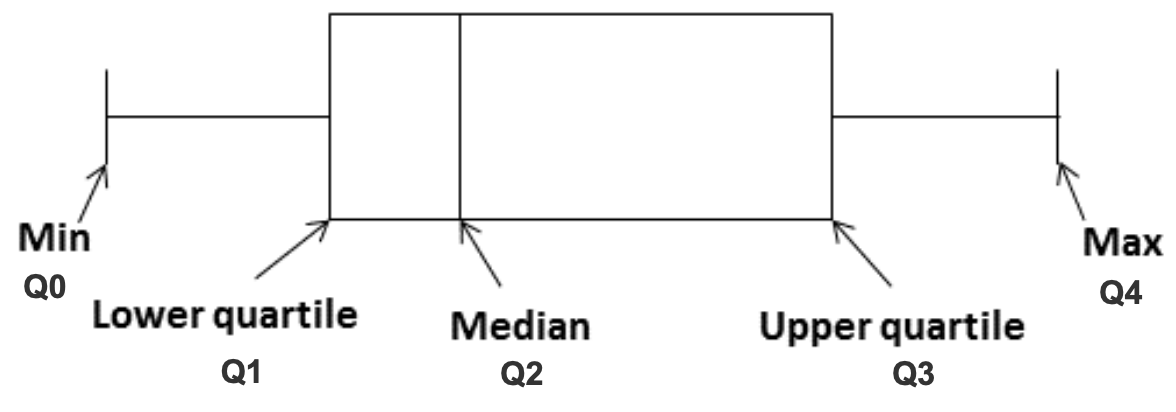
\includegraphics{../assets/boxplot.png}
    
    \paragraph{Skewness $\gamma$}

    \begin{tabular}{ l c c c }
        & Symmetric 
        & Left-Skewed
        & Right-Skewed \\
        
        Example
        & 
        & 
        &  \\
        
        Mean - Median 
        & Mean = Median
        & Mean < Median
        & Mean > Median \\
        
        Skewness $\gamma$
        & $\gamma$ = 0
        & $\gamma$ < 0
        & $\gamma$ > 0 \\
        
    \end{tabular}

    \paragraph{Kurosis Index $\beta$}  degree of peakedness of a distribution.
    $$
    $\beta$ = 0 \rightarrow normal distribution \\
    $\beta$ < 0 \rightarrow flat distribution \\
    $\beta$ > 0 \rightarrow peak distribution \\
    $$

    \section{Bivariate statistical analysis}
    
    \paragraph{Bivariate analysis} Analysis of two variables (X, Y), for the purpose of determining the empirical relationship between
    them. The bivariate statistical techniques vary according to the level of measurement
    of the crossed variables: Categorical Variables $\rightarrow$ Contingency table, Quantitative variables $\rightarrow$ Correlation

    \subsection{Contingency Tables}
    
    \paragraph{Contingency tables} The values in the  double-entry table are the
    absolute joint frequencies, and their sum is equal to the total of observed
    cases. The information may be used cell-wised (\textit{How many observation have this X and that Y? Probability that $X_i \cap Y_i$?}), 
    row wise (\textit{Across all X, what are the possible Y? Probability that $X_i$?}), 
    column wise (\textit{Accross all Y, what are the possible X? Probability that $Y_i$?})
    
    \paragraph{Marginal distributions} summing up per line and per column the joint frequencies
    \paragraph{Relative joint frequencies} The ratio between the absolute joint frequencies and the total of observed cases
    
    \subsection{Unidimensional distributions}
    
    \paragraph{Subordinate distributions} the frequency to observe the phenomenon x given
    the phenomenon y 
    $$P(X|Y) = \frac{P(X \cap Y)}{P(Y)}$$
    \paragraph{Statistical independence} Two events are statistically independent if the
    occurrence of one does not affect the probability of the other. The statistical independence is a symmetric concept: it is true for x, it true
    also for y. If it occurs, it means that the bivariate analysis does not provide
    additional information to the univariate analysis.
    $$P(X \cap Y) = P(X) \time P(Y)$$
    
    \paragraph{Chi-Square Hypothesis Testing} The Chi-Square can be computed by comparing the frequency that we would
    have in the case of perfect statistical independence between the two studied
    variables and the observed frequency. To do this,
    

    
\end{document}